\documentclass[12pt]{article}
\usepackage{geometry}
\geometry{a4paper, margin=1in}
\usepackage{graphicx}
\usepackage{amsmath}
\usepackage{listings}
\usepackage{xcolor}

\title{Network Architecture Design for MetroRail Transit Authority (MTA)}
\author{}
\date{}

\begin{document}

\maketitle

\section*{Introduction}
The rapid advancement of intelligent transportation systems has revolutionized the way railway networks operate, emphasizing the need for secure, efficient, and scalable network architectures. As the network architect for MetroRail Transit Authority (MTA), the task at hand is to design a state-of-the-art network infrastructure that supports an intelligent railway system spanning five major metropolitan cities in Bangladesh: Dhaka, Chittagong, Sylhet, Rajshahi, and Khulna.

Each city serves a unique role within the network, from Dhaka as the central operations hub managing over 10 railway stations, to Rajshahi acting as the disaster recovery and data redundancy center. The proposed system will integrate cutting-edge technologies such as IPv4 addressing for scalability, VLAN segmentation for traffic isolation, and SD-WAN for optimized interconnectivity between hubs. Additionally, robust security measures, including Zero Trust authentication and firewall policies, will ensure protection against cyber threats while maintaining operational reliability.
\section*{1. IPv4 Addressing Plan}

The IPv4 addressing scheme is designed to ensure scalability, efficiency, and security across all hubs and stations. Each regional hub and its associated railway stations are assigned unique subnets.

\subsection*{Subnet Breakdown}
\begin{itemize}
    \item \textbf{Dhaka (Main Branch)}:
    \begin{itemize}
        \item Central Operations Hub: $192.168.0.0/24$
        \item Railway Stations (10 stations): $192.168.1.0/24$ to $192.168.10.0/24$
        \item IoT Sensors, Surveillance Cameras, Ticketing Systems, and Passenger Wi-Fi: Subnets divided further into /26 blocks.
    \end{itemize}
    \item \textbf{Chittagong (South Maintenance Hub)}:
    \begin{itemize}
        \item Hub Network: $192.168.20.0/24$
        \item Railway Stations (5 stations): $192.168.21.0/24$ to $192.168.25.0/24$
    \end{itemize}
    \item \textbf{Sylhet (South-West Control Center)}:
    \begin{itemize}
        \item Hub Network: $192.168.30.0/24$
        \item Railway Stations (4 stations): $192.168.31.0/24$ to $192.168.34.0/24$
    \end{itemize}
    \item \textbf{Rajshahi (Disaster Recovery \& Data Redundancy Center)}:
    \begin{itemize}
        \item Hub Network: $192.168.40.0/24$
        \item Backup Data Storage: $192.168.41.0/24$
    \end{itemize}
    \item \textbf{Khulna (East Expansion \& Future Scaling)}:
    \begin{itemize}
        \item Hub Network: $192.168.50.0/24$
        \item Reserved for Future Stations: $192.168.51.0/24$ to $192.168.55.0/24$
    \end{itemize}
\end{itemize}

\subsection*{Scalability, Efficiency, and Security}
The hierarchical subnet structure ensures that each hub and station operates independently while maintaining connectivity. This design allows for easy addition of new stations and hubs without disrupting existing networks. VLAN segmentation further enhances security by isolating sensitive operational traffic from passenger services.

\section*{2. Network Diagram Description}

The network architecture consists of:
\begin{itemize}
    \item \textbf{Central Hub (Dhaka)}: Acts as the primary control center with connections to all regional hubs via SD-WAN.
    \item \textbf{Regional Hubs}: Chittagong, Sylhet, Rajshahi, and Khulna serve specific roles such as maintenance, control, disaster recovery, and future expansion.
    \item \textbf{SD-WAN Links}: Secure and optimized interconnectivity between hubs with QoS policies.
    \item \textbf{Firewalls}: Deployed at each hub to enforce access control and Zero Trust policies.
    \item \textbf{Redundancy Links}: Backup links ensure continuous operation during failures.
\end{itemize}

\begin{figure}[h]
    \centering
    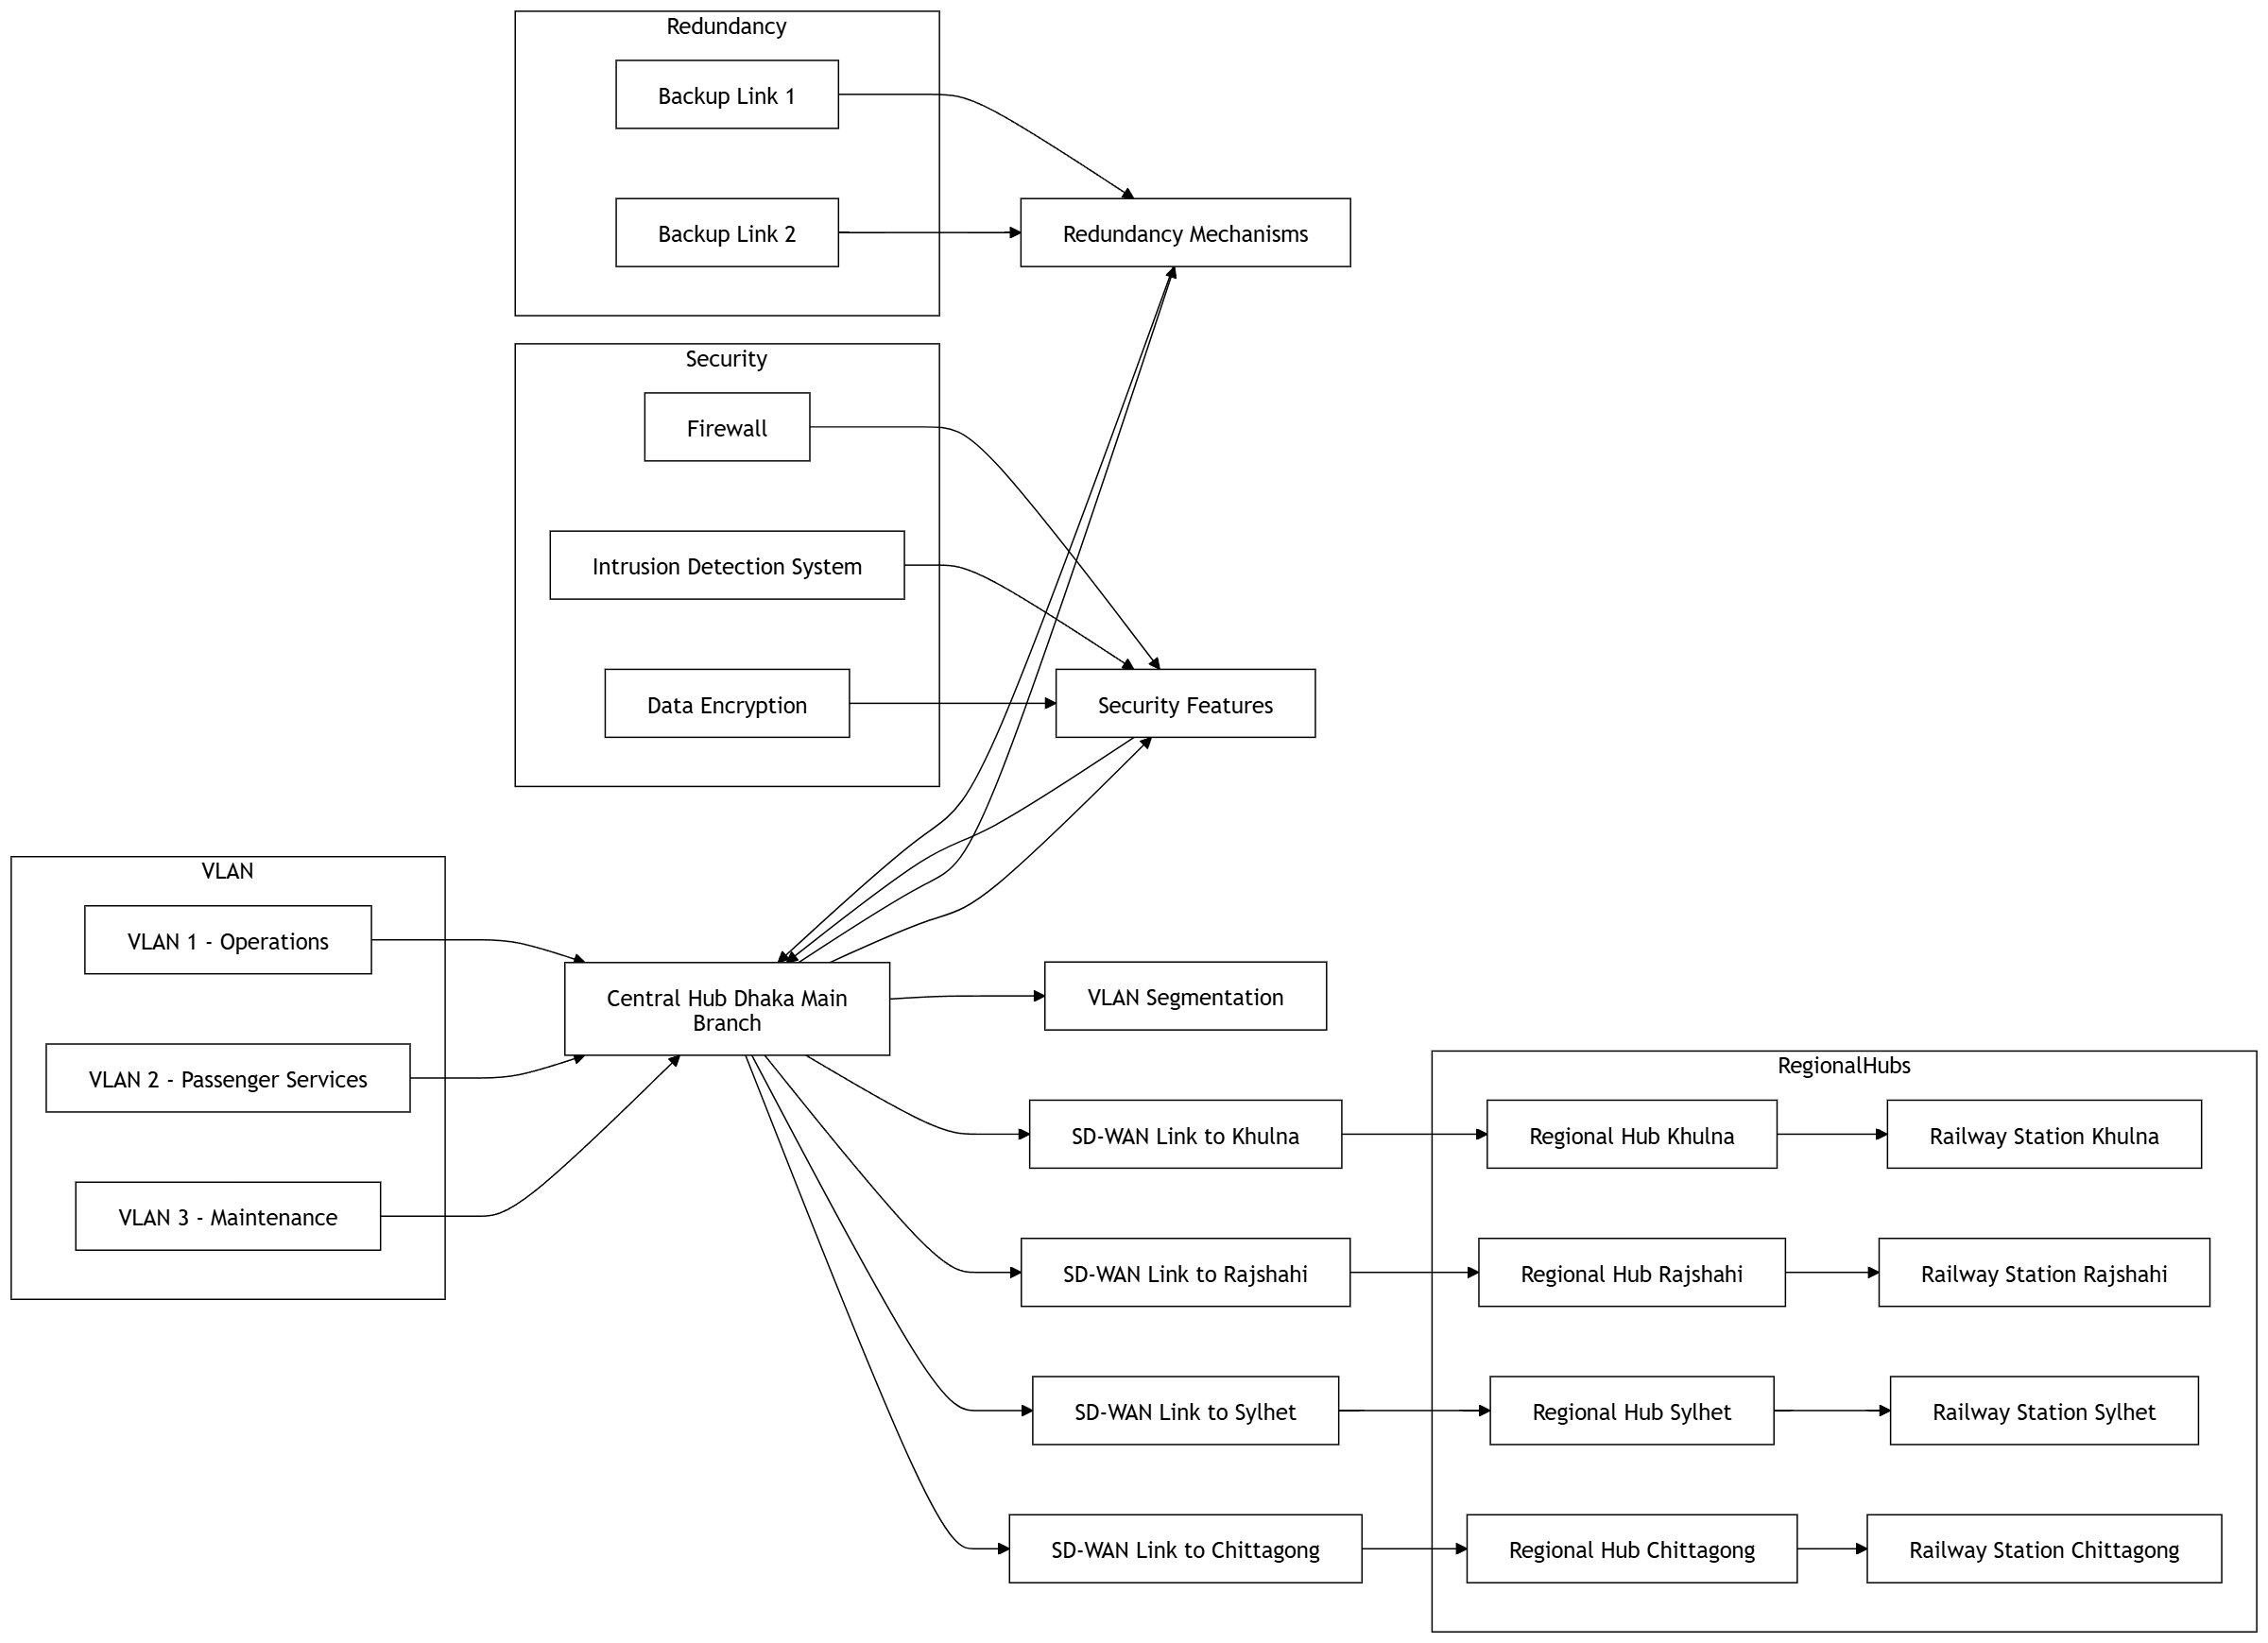
\includegraphics[width=1.0\textwidth]{./net3.png} 
    \caption{High-Level Network Architecture}
\end{figure}

\section*{3. SD-WAN Configuration Plan}

\subsection*{Traffic Prioritization Policies}
\begin{itemize}
    \item Train Control Data: Highest priority (Priority 1).
    \item Real-Time Tracking and Scheduling: Priority 2.
    \item Passenger Wi-Fi: Lowest priority (Priority 3).
\end{itemize}

\subsection*{Failover Mechanism}
\begin{itemize}
    \item Automatic failover is implemented using dual SD-WAN links.
    \item If the primary link fails, traffic is rerouted through a backup link with minimal disruption.
    \item Rajshahi serves as the disaster recovery site, ensuring data integrity and system availability.
\end{itemize}

\section*{4. Security and Firewall Configuration}

\subsection*{Firewall Policies}
\begin{itemize}
    \item Restrict external access to core railway operations.
    \item Whitelist specific traffic types (e.g., control data from Dhaka to Chittagong).
    \item Block unauthorized access to sensitive databases and systems.
\end{itemize}

\subsection*{Zero Trust Authentication}
\begin{itemize}
    \item All inter-region communication requires mutual authentication.
    \item Use certificates and multi-factor authentication (MFA) for secure access.
\end{itemize}

\section*{5. Justifications and Scalability Considerations}

\subsection*{Scalability}
The hierarchical subnet design allows for seamless addition of new stations and hubs. Reserved subnets in Khulna ensure future expansion.

\subsection*{Challenges}
\begin{itemize}
    \item \textbf{Cybersecurity}: Continuous monitoring and updates are required to mitigate evolving threats.
    \item \textbf{Bandwidth Management}: QoS policies ensure efficient use of available bandwidth.
    \item \textbf{Redundancy}: Backup links and disaster recovery mechanisms ensure high availability.
\end{itemize}

\section*{Conclusion}
The proposed network architecture meets the requirements for security, scalability, reliability, and efficiency. It leverages IPv6 adoption, VLAN segmentation, and SD-WAN to provide a robust foundation for MetroRail's intelligent railway system.

\end{document}